\hthree{Entwicklung}

Zunächst wurde für die Entwicklung eine separate NGINX-Konfiguration erstellt, die den Entwicklungsserver, der von Vite betrieben wird, an den Client weitergibt.

\css{code/Nginx/dev.conf}{NGINX-Konfiguration für die Entwicklung}

Um das Gesamtprojekt bereitzustellen, werden vier verschiedene Docker-Container gestartet.

Der erste ist die "MariaDB"-Datenbank, die alle Daten speichert. Der zweite ist die "API", die die Daten verwaltet und über unseren dritten Container, einen "NGINX"-Webserver, an die Webclients weiterleitet. Die Website selbst wird vom "Vite"-Entwicklungsserver bereitgestellt, der den vierten Container darstellt. 

\begin{figure}[H]
    \centering
    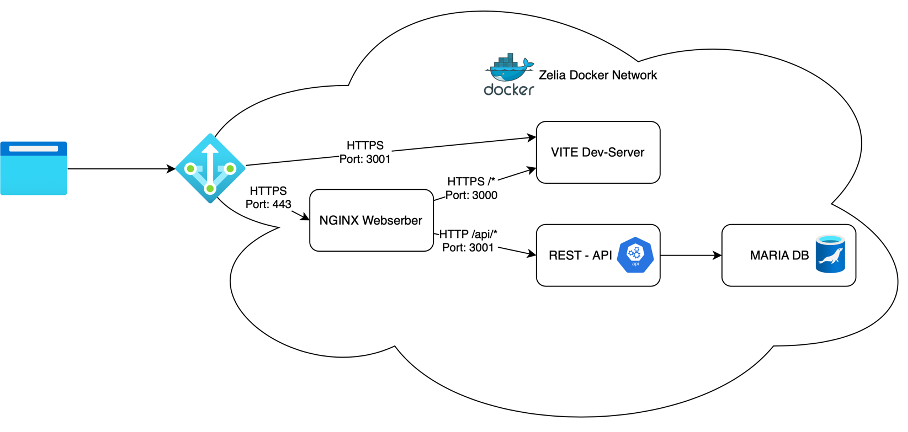
\includegraphics{media/Docker/DevNetwork.png}
    \caption{Docker-Netzwerk für die Entwicklung}
\end{figure}

Um das Datenbankschema aufzubauen und "Dummy"-Daten einzufügen, können SQL-Skripte im Verzeichnis /docker-entrypoint-initdb.d/ angelegt werden. Dort werden sie beim Start des Docker-Containers in alphabetischer Reihenfolge ausgeführt. Daher wurden sie mit Zahlen beginnend benannt, um die Reihenfolge festzulegen.

Um "Secrets" wie das Passwort zur Datenbank zu schützen, werden sie aus Umgebungsvariablen übernommen. Damit es nicht notwendig ist, die "Environment"-Variablen jedes Mal manuell zu setzten, ist es bei Docker möglich, eine "Env"-Datei anzugeben, die alle Umgebungsvariablen speichert. 
